\chapter{Differenze tra Initial Coin Offering e Security Token Offering}                %crea il capitolo
%%%%%%%%%%%%%%%%%%%%%%%%%%%%%%%%%%%%%%%%%imposta l'intestazione di pagina
\lhead[\fancyplain{}{\bfseries\thepage}]{\fancyplain{}{\bfseries\rightmark}}
\pagenumbering{arabic}
%mette i numeri arabi

\section{Storia delle monete elettroniche e delle criptomonete}

Sebbene le valute digitali abbiano raggiunto un nuovo livello di rilievo nel mondo solo negli ultimi anni, è importante ricordare che la monete elettroniche hanno una storia che risale a decenni fa. Il whitepaper \textit{“Bitcoin: A Peer-to-Peer Electronic Cash System”}\cite{K1}, pubblicato nel 2008 da un autore anonimo o da un gruppo di persone sotto lo pseudonimo di Satoshi Nakamoto, per quanto risulti innovativo e a posteriori anche rivoluzionario, si basa su tecnologie preesistenti e ben affermate tra le quali ad esempio le reti P2P, un fenomeno che ha radici nelle prime fasi della storia di Internet e reso popolare da Napster. Non sono solo le reti distribuite ad essere una fondazione per Bitcoin; nel whitepaper, Nakamoto si avvale infatti di altri lavori precedenti che risultano fondamentali al funzionamento della rete. Tra questi possiamo citare il lavoro di tesi pubblicato da Ralph Merkle nei primi anni ’70  riguardo alla comunicazione sicura attraverso canali insicuri e gli sviluppi apportati da Diffie e Hellman\cite{K2,K3}. Inoltre, è proprio a Merkle che dobbiamo l’invenzione dei Merkle Tree usati in Bitcoin poiché forniscono un metodo per firmare digitalmente messaggi contenuti in grandi strutture dati\cite{K4}. I merkle tree verranno successivamente ripresi da Bayer, Haber e Stornetta per la realizzazione efficiente di una catena di blocchi firmata crittograficamente\cite{K5}.


Altri lavori più recenti risultano essere punti chiave per lo sviluppo della rete Bitcoin ed in generale dei sistemi di pagamento elettronici.


Nel 1983 in \textit{“Blind Signatures for Untraceable Payments”} e nei sui lavori successivi\cite{K6,K7}, Chaum introduce l’idea di un sistema di pagamento elettronico anonimo basato sulla tecnologia di Blind Signature, sistema che verrà poi implementato dallo stesso autore con ECash™ nel 1994. Come osserva Schoenmakers\cite{K8} nonostante le istituzioni finanziare già utilizzassero dietro le quinte sistemi elettronici per processare transazioni l’apertura al pubblico dei sistemi di pagamento elettronici introduce la necessità di un sistema di pagamento elettronico che possa essere utilizzato in una rete ad accesso pubblico, particolarmente in riferimento alla rete Internet. Nel 1998 DigiCash fallisce, principalmente a causa della forte competizione posta in atto dal sistema di pagamento tramite carta di credito. Nel particolare secondo Chaum la compagnia ha sofferto di un chicken-and-egg problem: fu difficile convincere abbastanza venditori  ad adottare il sistema per  poter acquisire clienti e vice versa. (Lo stesso destino spetta ad altre forme di pagamento elettronico dello stesso periodo tra le quali possono essere citate CyberCoin, Virtual PIN. ) 


Sebbene infruttuosa, l’esperienza di Chaum rappresenta il primo esempio di un sistema di pagamento elettronico anonimo e risulta pionieristico sia nei problemi che vengono presentati come nelle soluzioni proposte, come avviene nel caso del problema di double spending. 


Altri sistemi di moneta digitale si sono susseguiti negli anni, tra i più rilevanti possiamo citare e-gold, Liberty Reserve e PayPal: I primi due non più attivi, entrambi per controversie legali, mentre l’ultimo ancora attivo. Questa lista non ha scopo di essere esauriente, per un approfondimento si rimanda alla letteratura relativa all'argomento.
Un altro tassello fondamentale nello sviluppo delle monete elettroniche è l’introduzione nel 1997 di hashcash\cite{K9} da parte di Adam Back che indipendentemente descrive un sistema simile a quanto proposto da Cynthia Dwork,  Moni Naor e Eli Ponyatovski nel 1992 in \textit{“Pricing via Processing or Combatting Junk Mail”}\cite{K10}. Entrambe le proposte prevedono l’utilizzo di quella che nel 1999 viene formalizzata da  Markus Jakobsson e Ari Juels come \textit{“proof of work”} per arginare il fenomeno dello spam\cite{K11}. Appena un anno prima, nel 1998, Wei Dai introduce B-money\cite{K12}, un sistema basato su hashcash che comprendeva varie funzionalità oggi comuni alla maggior parte delle criptomonete. B-money tuttavia non fu mai lanciato e rimase solo una proposta ma il lavoro di Dai non fu vano; dieci anni dopo, all'inizio dello sviluppo di Bitcoin, Dai fu il primo ad essere contattato da Nakamoto. A lui seguirono altri sviluppatori tra i quali Nick Szabo, creatore di bitgold, e Hal Finney, che introdusse l'idea di \textit{"reusable PoW"}\cite{K13}. 

Nel 1998 infatti, Nick Szabo creò bitgold\cite{K14}, un meccanismo per una digital currency decentralizzata e sicura che implementava già alcune idee alla base degli smart contracts. Le teorie di Szabo riguardo riguardo gli accordi auto-attuanti furono formulato all'incirca durante lo stesso periodo in cui Ian Grigg introdusse l'idea dei Ricardian Contract, un metodo per registrare un documento come un contratto legale e collegarlo in modo sicuro ad altri sistemi\cite{K15}. Bitgold, come B-money, non fu mai implementato.

\subsection{Creazione e diffusione di Bitcoin}

La pubblicazione del whitepaper di Bitcoin avviene finalmente nel 2008, poco dopo il clou della crisi finanziaria e del collasso di Lehman Brothers. L'obbiettivo a cui Bitcoin mira è fornire una valuta digitale P2P che non necessiti della presenza di banche ed altri intermediari.  La prima implementazione di bitcoin fu opera di Nakamoto ma successivamente la direzione dei lavori passò gradualmente ad un gruppo di primi utenti e sviluppatori capitanati da Gavin Andersen. 

E' interessante notare come nel suo whitepaper\cite{K1} Nakamoto non si riferisca a \textit{"blockchain"} ma solo a \textit{"chain of blocks"}. Il termine \textit{"blockchain"} infatti si diffonde successivamente durante lo sviluppo di protocolli alternativi a bitcoin. 

Dalla sua creazione nel 2008 fino ad oggi il prezzo di acquisto per un bitcoin è passato da  0.003\$, il valore della prima quotazione su un exchange dedicato, fino al valore massimo di circa 19000\$ come è possibile osservare nella figura \ref{fig:chartbitcoin}. A questo valore è stato stimato che il patrimonio di Nakamoto abbia raggiunto un valore di 19 miliardi di dollari, dato che possiede circa un milione di bitcoin, o più. Nonostante ciò, dalla sua uscita di scena nel 2011 Nakamoto non ha operato transazioni con i bitcoins di cui sappiamo essere in possesso. 
\begin{figure}[H]
  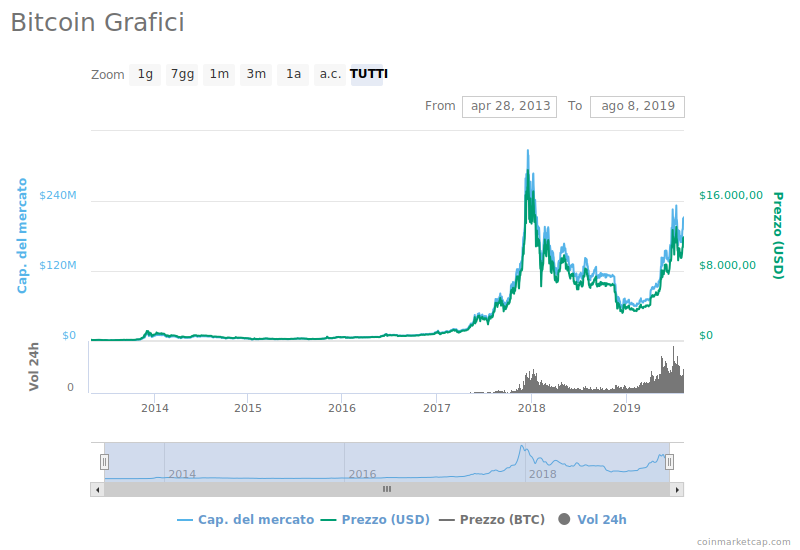
\includegraphics[width=\linewidth]{chartbitcoin.png}
  \caption{Grafico di prezzo di Bitcoin}
  \label{fig:chartbitcoin}
\end{figure}

Il codice open source di Bitcoin ha permesso ad altri sviluppatori di creare protocolli alternativi\cite{K16}, in questo periodo infatti si assiste alla nascita di quelle che verranno in seguito definite \textit{"Altcoin"}, un'abbreviazione di \textit{"alternative coin"}. Allo stesso tempo si inizia a diffondere anche l'utilizzo di Bitcoin in alcune organizzazioni, tra le prime possiamo citare Wikileaks e Electronic Frontier Foundation. Nel 2011 viene pubblicato il sito tematico Bitcoin Magazine che tra i suo fondatori annovera anche Vitalik Buterin. Nel 2012 la Bitcoin Foundation inizia i propri sforzi di standardizzazione e promozione di Bitcoin. Nello stesso anno BitPay, un azienda che offre servizi di pagamento tramite bitcoin riporta che più di 1000 commercianti avevano adottato il suo sistema di pagamento. Nel 2013, Coinbase, un'altra azienda per il processo dei pagamenti tramite bitcoin, annuncia di aver venduto bitcoin per un valore pari a 1 milione di dollari in un mese, ad un prezzo di circa 22\$ per unità. 
A questo punto, l'utilizzo di bitcoin entra nei radar degli enti regolatori a causa di una alta volatilità dovuta a diversi fattori concorrenti. L'American Financial Crimes Enforcement Network (FinCEN) stabilisce delle linee guida per monete virtuali decentralizzate, con particolare riferimento a Bitcoin, introducendo l'obbligo per i miners di essere registrati come Money Service Business (MSBs) qualora vendessero i bitcoin generati\cite{K17}. Anche altri enti americani entrano in contatto con bitcoin durante incidenti ed indagini, come ad esemplificato da un avviso di sequestro emesso dalla Drug Enforcement Agency (DEA) per 11 bitcoins. Non a caso, a partire dal 2013 si può osservare una divergenza nelle regolamentazioni implementate da diversi stati. 
Tra gli esempi più rilevanti possiamo citare il caso tailandese: il Foreign Exchange Administration and Policy Department sancisce che il bitcoin è illegale data l'assenza di un framework legale al quale possa essere sottoposto\cite{K18}. Il 2013 risulta essere un anno saliente per bitcoin anche per un altro aspetto. La Cina diventa infatti il più grande punto di scambio di bitcoin. Tuttavia la Banca Popolare Cinese (PBC o PBOC) proibisce l'uso di Bitcoin agli istituti finanziari cinesi, causando in dicembre un crollo dei prezzi\cite{K19}. 

Nel 2014 emergono prodotti derivati basati su Bitcoin, approvati dall'U.S.Commodity Futures Trading Commission come prodotti di scambio over-the-counter che hanno come sottostante il prezzo del bitcoin. Inoltre, aumentano i casi di furto elettronico di bitcoin, di particolare rilievo risultano essere i casi di Mt Gox e Bitstamp. 
Da qui in poi l'espansione globale di Bitcoin continua inesorabilmente, nonostante le incertezze della mutevole configurazione giuridica nei diversi stati, grazie anche ad una tendenza di regolamentazione più favorevole.  

\subsection{Creazione e diffusione di Ethereum}

Ethereum viene descritto in un whitepaper\cite{K20} da Vitalik Buterin, verso la fine del 2013.
Vitalik riporta che durante l'ottobre del 2013 lavorando in Israele a contatto con il team di Mastercoin, in \textit{"Utimate Scripting"} avanza delle proposte per generalizzare il protocollo utilizzato da Mastercoin. Queste proposte risultano abbastanza distanti dalle funzionalità di Ethereum, rappresentano infatti una prima versione di un protocollo finalizzato solo alla creazione di un contratto tra due parti nelle quali il valore monetario viene redistribuito secondo una formula specificata nel contratto stesso. Sebbene impressionato, il team di Mastercoin decise di non implementare le modifiche proposte. In Dicembre Buterin propone una nuova versione, la prima che adotta il nome Ethereum e che presenta una generalizzazione degli smart contracts. In questa versione invece di utilizzare un linguaggio di scripting per descrivere i termini di una relazione tra due parti, gli smart contracts sono account veri e propri, con la possibilità di possedere, spedire e ricevere assets\cite{K21}. Da questo momento in poi Ethereum attira l'interesse di altri sviluppatori, primi tra i quali Gavin Wood, Jeffrey Wilcke, Andrew Miller, Mihai Alisie, Anthony Di Iorio e Charles Hoskinson. 
Ethereum viene formalmente annunciato il 25 Gennaio 2014 a Miami durante la North America Bitcoin Conference  e nell'estate del 2014 dopo i primi lavori degli sviluppatori il protocollo si stabilizza, quindi Wood pubblica una specifica semi-formale di Ethereum e dell'Ethereum Virtual Machine\cite{K22}. Intanto altri sviluppatori si aggiungono al progetto ed anche alcuni finanziatori decidono di prendervene parte.
Parallelamente a queste prime fasi di sviluppo vengono formate diverse entità legali per poter coordinare il progetto, in particolare Ethereum Switzerland GmbH (EthSuisse) e Ethereum Foundation (Stiftung Ethereum). Lo sviluppo fu finanziato tramite crowdfounding, vendendo il token di ethereum, denominato ether, in cambio di bitcoin. Grazie alla crowdsale, 11,9 milioni di ether furono venduti, per un valore di circa 18,4 milioni di dollari. 

Sin dal suo lancio iniziale, Ethereum ha ricevuto numerosi aggiornamenti pianificati del proprio protocollo, con cambiamenti importanti per quanto riguarda le funzionalità dello stesso. 
A testimonianza del successo del progetto Ethereum, nel marzo 2017, varie startups, gruppi di ricerca e aziende appartenenti alla Fortune 500 hanno annunciato la creazione della Enterprise Ethereum Alliance (EEA) con trenta membri fondatori. 
In maggio, l'organizzazione no-profit conta 116 membri, includendo ConsenSys, CME Group, Cornell University's research group, Toyota Research Institute, Samsung SDS, Microsoft, Intel, J. P. Morgan, Cooley LLP, Merck KGaA, DTCC, Deloitte, Accenture, Banco Santander, BNY Mellon, ING, and National Bank of Canada.
In Luglio il numero di membri raggiunge i 150, tra i quali MasterCard, Cisco Systems, Sberbank and Scotiabank. Altri membri di rilevo sono Advanced Micro Devices (AMD), FedEx Corporate Services, Hyperledger, Securitize, TOKENY, UniCredit e VMware.

\section{Le criptomonete come strumento di finanziamento}
Come già accennato, inizialmente Ethereum ricevette finanziamenti tramite una crowdsale sulla rete Bitcoin.  Questo ha permesso agli sviluppatori di intercettare l'interesse degli utenti disposti a supportare lo sviluppo della piattaforma. Tuttavia, la prima token sale avvenne nel luglio 2013 grazie a J.R. Willett con lo scopo di raccogliere fondi per il progetto Omni tramite la vendita di Mastercoin\cite{K23}. Per motivare i potenziali investitori a contribuire al progetto, Willet fece in modo di rendere disponibile molte delle funzioni solo ai possessori di mastercoins. Fu quindi Willet ad ideare il modello delle ICO ed a lui dobbiamo anche l'introduzione di quelli che successivamente verranno definiti come utility token. La token sale permise a Willet di raccogliere finanziamenti per un valore di 600 mila dollari, al tempo circa 4740 bitcoin. Il protocollo introdotto con mastercoin, oggi chiamato \textit{"Omni Layer"}, ha avuto molto successo tanto da essere usato come protocollo su cui si basa il token Tether (USDT), ad oggi una delle criptomonete più scambiate dopo il bitcoin\cite{K24}. 
Il secondo token venduto tramite ICO è NextCoin (NXT), che tra settembre ed ottobre del 2013 permette al suo creatore, rimasto anonimo, di raccogliere 21 bitcoin, per un valore compreso tra i 3000 e 17000 dollari. A NextCoin seguono Counterparty (XCP), MaidSafeCoin (MAID), Swarm e successivamente Ethereum.\cite{K25,K26,K27,K28}

Poiché Ethereum è pensata come una piattaforma per la creazione ed esecuzione di smart contracts e grazie alla possibilità di sviluppare token sulla piattaforma stessa, risulta ovvio il perché Ethereum sia diventata la piattaforma più usata per ospitare altre crowdsale. La prima Initial Coin Offering (ICO) basata sulla piattaforma Ethereum fu lanciata il 17 Agosto 2015, per la vendita di token Augur\cite{K29}. La vendita durò fino al 5 Settembre dello stesso anno. In seguito alla vendita vennero raccolti più di 5 milioni di dollari per lo sviluppo del progetto Augur. Il progetto è stato lanciato ufficialmente nel luglio del 2018. 

Il fenomeno delle ICOs è via via diventato popolare con un picco nel 2017. Dall'inizio  del 2017 fino ad ottobre 2017 infatti, vengono raccolti fondi per un valore di 2,3 miliardi di dollari, un risultato dieci volte maggiore rispetto al 2016. 
Durante tutto il 2017 vengono raccolti fondi per un valore di circa 6 miliardi di dollari, il 37\% dei quali dovuti a solamente 20 ICO. 

\begin{figure}[H]
  \includegraphics[width=\linewidth]{ico.jpg}
  \caption{ICO data, source: Florie Mazzorana-Kremer\cite{K30}}
  \label{fig:ico}
\end{figure}

Viene stimato che al Febbraio 2018 il 46\% delle progetti finanziati tramite una ICO nel 2017 sono falliti. 

\section{Classificazione dei token nelle token sales}
Comunemente, in base alla sua funzione, un token venduto in una token sale può essere considerato un utility token, un security token o un currency token. Questa distinzione è comunemente riconosciuta ed è adottata anche dalla Swiss Financial Market Supervisory Authority (FINMA). In particolare si riporta quanto segue:

\textit{‘‘Asset tokens represent assets such as participations in real physical underlyings, companies, or earnings streams, or an entitlement to dividends or interest payments. In terms of their economic function, the tokens are analogous to equities, bonds or derivatives.While, Utility tokens are tokens which are intended to provide digital access to an application or service.’’}


Un currency token, come ad esempio il bitcoin, rappresenta una valuta digitale ed è quindi un mezzo di scambio.

Un utility token è usato all'interno di una rete per poter accedere ad una funzionalità o per il funzionamento di questa. 
I security tokens si riferiscono ad una rappresentazione digitale tramite blockchain di securities. La definizione di security tuttavia varia a seconda della legislazione applicabile.
Negli Stati Uniti le securities sono definite nell'U.S. Code of Laws 15 §77b(a)(1) come:

\textit{‘‘The term ‘‘security’’ means any note, stock, treasury stock, security future, bond, debenture, evidence of indebtedness, certificate of interest or participation in any profit sharing agreement, collateral-trust certificate, preorganization certificate or subscription, transferable share, investment contract, voting-trust certificate, certificate of deposit for a security, fractional undivided interest in oil, gas, or other mineral rights, any put, call, straddle, option, or privilege on any security, certificate of deposit, or group or index of securities (including any interest therein or based on the value thereof), or any put, call, straddle, option, or privilege entered into on a national securities exchange relating to foreign currency, or, in general, any interest or instrument commonly known as a ‘‘security’’, or any certificate of interest or participation in, temporary or interim certificate for, receipt for, guarantee of, or warrant or right to subscribe to or purchase, any of the foregoing.’’}

In particolare, per quanto concerne le STOs queste devono aderire ad una delle seguenti normative: Regulation D, Regulation A+ o Regulation S\cite{K31,K32,K33}. 

In Italia l'equivalente delle securities sono gli strumenti finanziari definiti nel D.lgs 24 febbraio 1998 n.58, noto come testo unico della finanza, abbreviato in TUF o legge Draghi\cite{K34}. Ad oggi in Italia vi sono ulteriori linee guida riguardanti la configurazione da adottare per il pagamento di imposte e in materia di antiriciclaggio. Inoltre, con l'introduzione nel nostro ordinamento delle tecnologie DLT e Smart Contract, come previsto dalla legge 12/2019 di conversione del D.L. n. 135/2018, l'emissione di security tokens da parte di soggetti in possesso dei requisiti necessari è teoricamente possibile, nonostante nessuna STO sia stata realizzata fino ad oggi in Italia.

Alcune legislazioni si sono espresse con linee guida specifiche applicabili ai security token, come ad esempio la Financial Conduct Authority (FCA) in UK che nel Gennaio 2019 ha indicato la differenza tra security e utility token come segue:

\textit{“Security tokens are tokens with specific characteristics that mean they meet the definition of a Specified Investment like a share or a debt instrument as set out in the Regulated Activities Order, and are within the perimeter.
While, utility tokens grant holders access to a current or prospective product or service but do not grant holders rights that are the same as those granted by Specified Investments.”}

Da questo punto di vista le Security Token Offerings (STOs) sono l'evoluzione naturale delle ICOs. Questa evoluzione è dovuta alla necessità per le aziende di operare nel settore delle criptomonete definendo con chiarezza le normative da rispettare. Lo scopo delle STOs infatti è esclusivamente quello di creare token equiparabili a securities. In questo modo, configurandosi come securities, viene aggirato il vuoto normativo o l'incompletezza legislativa ancora presente in vari stati. E' infatti vantaggioso per un azienda trattare un token come una securities poiché ci si configura in un ambito normativo già consolidato e di cui molti professionisti hanno già esperienza. In definitiva, se le ICOs hanno avuto modo di proliferare grazie al vuoto normativo sulle criptomonete, le STOs puntano a diffondersi grazie al fatto di consistere in una vendita di strumenti finanziari rappresentati in forma digitale. La distinzione principale tra una ICO e una STO risulta appunto essere il ruolo del token e della regolamentazione. Una STO può offrire solamente security tokens e deve essere regolamentata. Una ICO, invece, non può offrire un security token poiché vi è nessuna regolamentazione. Non a caso, durante il 2018 la SEC ha sanzionato varie aziende per aver offerto securities tramite ICO non regolamentate. 
L'approccio delle STOs si basa sull'idea che una security non è definita dal mezzo con la quale essere viene rappresentata, ponendo quindi un'equivalenza tra un documento cartaceo e uno digitale grazia alla definizione legislativa che è nella maggior parte dei casi agnostica rispetto alla tecnologia.  Da questo punto di vista l'approccio comunemente adottato è quello di operare in una singola legislazione oppure operare in legislazioni diverse facendo attenzione a soddisfare ai requisiti imposti. Quest'ultimo caso richiede uno sforzo nettamente maggiore rispetto al primo; Operando in una sola legislazione è possibile gestire la maggior parte dei requisiti in modo automatico, o molto agevolato, attraverso l'implementazione di uno smart contracts dedicato. Operando in legislazioni diverse, l'implementazione dello smart contract deve essere compatibile per più legislazioni con il rischio di essere troppo generico o troppo specifico. In entrambi i casi non è ancora presente un meccanismo di automatic compliance. Alla singola azienda è quindi richiesto produrre la documentazione legalmente richiesta e di assolvere agli obblighi normativi. Allo stesso tempo è compito dell'azienda assicurarsi di essere autorizzata all'emissione di securities. Ovviamente il maggiore sforzo richiesto all'issuer della securities si traduce in un maggiore costo rispetto ad un ICO. Tuttavia, il maggiore costo permette all'azienda di ridurre il rischio di contenziosi legali e di evitare la possibilità di sanzioni. 
In un articolo pubblicato recentemente, Ante e Fielder\cite{K35} sostengo l'idea che le STOs siano più adatte delle ICOs nel soddisfare i bisogni di un'azienda e degli investitori. Oltre alla chiarezza normativa vengono citati come argomenti la possibilità di trasferimento istantaneo, un mercato secondario attivo 24/7, l'eliminazione della figura del broker riducendo di conseguenza i costi ed infine la trasparenza e sicurezza fornite dell'utilizzo della tecnologia blockchain.\cite{K30} Altri vantaggi che si sostiene vengano offerti dalle STOs sono la possibilità di implementare pagamenti automatici per realizzare un meccanismo di pagamento dei dividendi e la  frazionabilità della security\cite{K36}. In seguito in questo elaborato si andrà a verificare e obbiettare alcuni di questi pretese.  

Per riassumere, nella tabella \ref{tab:stoico} possiamo confrontare le caratteristiche delle ICOs e delle STOs.  
\begin{table}[]
\begin{tabular}{ccc}
\hline
 & \begin{tabular}[c]{@{}c@{}}Initial Coin Offering \\ (ICO)\end{tabular} & \begin{tabular}[c]{@{}c@{}}Security Token Offering \\ (STO)\end{tabular} \\ \hline
\multicolumn{1}{c|}{Periodo di successo} & 2017 & 2018 \\
\multicolumn{1}{c|}{Investitori} & \begin{tabular}[c]{@{}c@{}}Copertura globale,\\ barriere all'entrata minime\end{tabular} & \begin{tabular}[c]{@{}c@{}}Solo autorizzati, \\ barriere all'entrata\end{tabular} \\
\multicolumn{1}{c|}{\begin{tabular}[c]{@{}c@{}}Capitale\\  richiesto\end{tabular}} & \begin{tabular}[c]{@{}c@{}}Capitale minimo, \\ processo automatizzato\end{tabular} & \begin{tabular}[c]{@{}c@{}}Capitale medio-basso,\\ più efficienti di una security\\ tradizionale\end{tabular} \\
\multicolumn{1}{c|}{Regolamentazione} & Non regolamentate & \begin{tabular}[c]{@{}c@{}}Regolamentate in base alla \\ giurisdizione applicabile\end{tabular} \\
\multicolumn{1}{c|}{Token} & Qualsiasi tipo di token & Security (equity, asset, ecc) \\
\multicolumn{1}{c|}{Garanzie} & A discrezione dell'azienda & \begin{tabular}[c]{@{}c@{}}Diritti legali,\\ sorveglianza dei regolatori\\ e auditing aziendale\end{tabular} \\ \hline
\end{tabular}
\caption{Confronto tra ICOs e STOs}
\label{tab:stoico}
\end{table}